\documentclass[aspectratio=169, xcolor=dvipsnames]{beamer}
\usetheme{Simple}

\usepackage{subcaption}
\usepackage{amsfonts}
\usepackage{amsmath}
\usepackage{version}
\usepackage{tikz}
\usepackage{graphicx}
\usepackage{pgfplots}
\usepackage{caption}
\usepackage{array}
\usepackage{dsfont}
\usepackage{esvect}
\usepackage[backend=bibtex]{biblatex}
\usepackage[english]{babel}
\usepackage{csquotes}
\usepackage[T1]{fontenc}
\usepackage{braket}
\usepackage{hyperref}
\usepackage{float}
\usepackage{url}
\usepackage{stmaryrd}
\usepackage{xargs}
\usepackage{tensor}
\usepackage{tcolorbox}
\usepackage[separate-uncertainty = true,multi-part-units=single]{siunitx}
\usepackage[compat=1.1.0]{tikz-feynman}
%\usepackage{enumitem}

\usetikzlibrary{shapes,backgrounds}
\usetikzlibrary {shapes.symbols}


% better underbrace ==============================================

\usetikzlibrary{decorations.pathreplacing}
\makeatletter
\def\underbrace#1{%
	\@ifnextchar_{\tikz@@underbrace{#1}}{\tikz@@underbrace{#1}_{}}}
\def\tikz@@underbrace#1_#2{%
	\tikz[baseline=(a.base)] {\node[inner sep=0] (a) {\(\displaystyle #1\)};
		\draw[line cap=round,decorate,decoration={brace,amplitude=5pt}]
		(a.south east) -- node[below,inner sep=7pt] {\(\scriptstyle #2\)} (a.south west);}}
\def\overbrace#1{%
	\@ifnextchar^{\tikz@@overbrace{#1}}{\tikz@@overbrace{#1}^{}}}
\def\tikz@@overbrace#1^#2{%
	\tikz[baseline=(a.base)] {\node[inner sep=0] (a) {\(#1\)};
		\draw[line cap=round,decorate,decoration={brace,amplitude=5pt}]
		(a.north west) -- node[pos=.5,above,inner sep=7pt] {\(\scriptstyle #2\)} (a.north east);}}
\makeatother


% color box ==============================================================
\usepackage{xcolor}

% Syntax: \colorboxed[<color model>]{<color specification>}{<math formula>}
\newcommand*{\colorboxed}{}
\def\colorboxed#1#{%
	\colorboxedAux{#1}%
}
\newcommand*{\colorboxedAux}[3]{%
	% #1: optional argument for color model
	% #2: color specification
	% #3: formula
	\begingroup
	\colorlet{cb@saved}{.}%
	\color#1{#2}%
	\boxed{%
		\color{cb@saved}%
		#3%
	}%
	\endgroup
}

% miscellaneous commands

\newcommand{\dd}[2]{\frac{\mathrm{d}#1}{\mathrm{d}#2}}
\newcommand{\dpart}[2]{\frac{\partial#1}{\partial#2}}
\newcommandx{\intg}[4][2=,3=,4=]{\int\IfValueT{#3}{_{#3}}\IfValueT{#4}{^{#4}}\mathrm{d}\IfValueT{#2}{^{#2}}#1\hspace{1mm}}
\newcommand{\feynint}[1]{\int\frac{\mathrm{d}^D#1}{\left(2\pi\right)^D}}
\newcommand{\LL}{\mathrm{L}}
\newcommand{\RR}{\mathrm{R}}
\usetikzlibrary{positioning,calc,angles,quotes}

\title{The Transverse Field Ising Model}
\subtitle{Monte-Carlo simulation of Quantum Phase Transitions}
\author{Mathieu Ferey}
\date{22/12/2023}
\titlegraphic{
\includegraphics[height=2cm]{Images/eth_logo.png}}

\addbibresource{biblio.bib}

% table of content at each section ========================================================
\AtBeginSection[]
{
	\begin{frame}
		\frametitle{Table of Contents}
		\tableofcontents[currentsection]
	\end{frame}
}

% better title page ===========================================================
\setbeamertemplate{title page}[default][colsep=-4bp,rounded=false]

\begin{document}
	
\frame{\titlepage}
	
\begin{frame}{Contents}
	\tableofcontents
\end{frame}


\section{Theoretical background}

\begin{frame}{$\mathds{Z}_2$ gauge theory}
	
	\begin{columns}
		
		\column{0.5\textwidth}
		
		\begin{itemize}
		
		\item $\mathds{Z}_2$ gauge theory Hamiltonian on a 2D lattice
		\vspace{-3mm}
		\begin{multline*}
			H_{\mathds{Z}_2} = -g\sum_{\vec{x},j}\sigma^x_j(\vec{x})\\ -\frac{1}{g}\sum_{\vec{x}}\sigma_1^z(\vec{x})\sigma_2^z(\vec{x}+e_1)\sigma_1^z(\vec{x}+e_2)\sigma_2^z(\vec{x}),
		\end{multline*}
		
		\onslide<2>{
		\item Duality with a Transverse Field Ising model on the 2D dual lattice 
		\vspace{-2mm}
		\begin{equation*}
			H = -g\sum_{\vec{r},j}\tau^z(\vec{r})\tau^z(\vec{r}+e_j) - \frac{1}{g}\sum_{\vec{r}}\tau^x(\vec{r}).
		\end{equation*}}
	
		\end{itemize}
	
		\column{0.5\textwidth}
	
		\begin{figure}
			\centering
			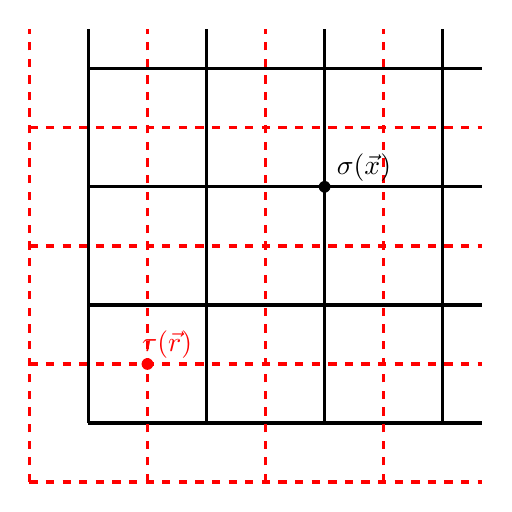
\begin{tikzpicture}
				\draw [step=1.5, black, very thick] (0,0) grid (5,5);
				
				\onslide<2>{\draw [dashed, very thick, red, step=1.5cm, xshift=-0.75cm, yshift=-0.75cm] (0,0) grid +(5.75,5.75);
				
				\node at (0.75,0.75)[red,circle,fill,inner sep=1.5pt]{};
				\node[red] (tau) at (1,1){$\tau(\vec{r})$};}
				
				\node at (3,3)[black,circle,fill,inner sep=1.5pt]{};
				\node[black] (sigma) at (3.5,3.25){$\sigma(\vec{x})$};
				
			\end{tikzpicture}
		\end{figure}

	\end{columns}

\end{frame}


\begin{frame}{The Transverse Field Ising model}
	
	\begin{equation*}
		H = -J\sum_{\langle i,j\rangle} S_i^zS_j^z - \Gamma\sum_i S_i^x	
	\end{equation*}


	\begin{equation*}
		\left[S^z,S^x\right] = iS^y,\hspace{1cm} S^z\ket{\pm 1} = \pm\ket{\pm 1},\hspace{1cm} S^x\ket{\pm 1} = \ket{\mp 1}
	\end{equation*}

	\vspace{1cm}
	\centering
	\textbf{A quantum Hamiltonian requires a quantum treatment!}

\end{frame}


\begin{frame}{Classical Mapping: a proof in 1D}

	From the Hamiltonian
		
	\begin{equation*}
		H = -J\sum_{i=1}^N S_i^zS_{i+1}^z - \Gamma\sum_{i=1}^N S_i^x,		
	\end{equation*}

	compute the partition function

	\begin{equation*}
		Z = \mathrm{Tr}\exp\left(-\beta H\right) = \mathrm{Tr}\exp\left(-\beta\left(H_0+V\right)\right).
	\end{equation*}
	
	\onslide<2>With the Trotter formula \cite{trotter}
		
	\begin{equation*}
		\exp\left(A_1+A_2\right) = \lim_{M\to\infty}\left[\exp\left(A_1/M\right)\exp\left(A_2/M\right)\right]^M,
	\end{equation*}
		
	expand the partition function
	
	\begin{equation*}
		Z = \sum_{\left\{S^1_1,\cdots,S^1_N\right\}}\bra{S^1_1,\cdots,S^1_N}e^{-\beta H_0/M}e^{-\beta V/M}\times\cdots\times e^{-\beta H_0/M}e^{-\beta V/M}\ket{S^1_1,\cdots,S^1_N}.
	\end{equation*}

\end{frame}

\begin{frame}
	
	\begin{align*}
		Z &= \sum_{\left\{S^1_1,\cdots,S^1_N\right\}}\bra{S^1_1,\cdots,S^1_N}e^{-\beta H_0/M}e^{-\beta V/M}\times\cdots\times e^{-\beta H_0/M}e^{-\beta V/M}\ket{S^1_1,\cdots,S^1_N}\\
		&= \sum_{\left\{S\right\}}\prod_{k=1}^M\bra{S^k_1,\cdots,S^k_N}e^{-\beta H_0/M}e^{-\beta V/M}\ket{S^{k+1}_1,\cdots,S^{k+1}_N}\\
		\onslide<2>{&= \left(\frac{1}{2}\sinh(2\beta\Gamma/M)\right)^{MN/2}\sum_{\left\{S\right\}}\exp\left[-\frac{\beta}{M}\left(-J\sum_{i=1}^N\sum_{k=1}^M S_i^k S_{i+1}^k\right.\right.\\
		&\hspace{5cm}-\left.\left. \frac{M}{2\beta}\ln\coth\left(\dfrac{\beta\Gamma}{M}\right)\sum_{i=1}^N\sum_{k=1}^M S_i^k S_i^{k+1}\right)\right]}
	\end{align*}
	
\end{frame}


\begin{frame}{Classical mapping in 1D}
	
	\begin{equation*}
		H = -J\sum_{i=1}^N S_i^zS_{i+1}^z - \Gamma\sum_{i=1}^N S_i^x,		
	\end{equation*}
	\vspace{-6mm}
	\begin{figure}
		\centering
		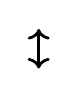
\begin{tikzpicture}[anchor=center]
			\draw[<->,line width=1](0,0) to (0,-0.5);
		\end{tikzpicture}
	\end{figure}
	\vspace{-3mm}
	\begin{equation*}
		H_\mathrm{eff} = -J\sum_{i=1}^N\sum_{k=1}^M S_i^k S_{i+1}^k - \frac{M}{2\beta}\ln\coth\left(\dfrac{\beta\Gamma}{M}\right)\sum_{i=1}^N\sum_{k=1}^M S_i^k S_i^{k+1},
	\end{equation*}

	\vfill
	
	\onslide<2>\begin{tcolorbox}[colback=blue!5!white,colframe=DarkBlue]
		\centering
		\textbf{Classical thermal phase transitions in $d+1$ dimensions}\\ 
		$\downarrow$\\
		\textbf{Quantum phase transitions in $d$ dimensions}
	\end{tcolorbox}

	
\end{frame}


\begin{frame}{Classical mapping in 2D}
	
	The quantum Hamiltonian on a 2D $N_x\times N_y$ lattice
		
	\begin{equation*}
		H = -J\sum_{i,j}S^z_{i,j}\left(S^z_{i+1,j} + S^z_{i,j+1}\right) -\Gamma\sum_{i,j}S^x_{i,j},
	\end{equation*}
	
	can be mapped to a classical anisotropic Ising model on a 3D $N_x\times N_y \times N_z$ lattice
	
	\begin{equation*}
		H_\mathrm{eff} = -\sum_{k=1}^{N_z}\sum_{i,j}\left[J S_{i,j,k}\left(S_{i+1,j,k} + S_{i,j+1,k}\right) + K_{N_z}(\beta) S_{i,j,k}S_{i,j,k+1}\right].
	\end{equation*}
	
\end{frame}


\begin{frame}{Phase transitions}
	
	\begin{columns}
		
		\column{0.5\textwidth}
		
		\textbf{Two phases}
		\begin{center}
			
			\begin{itemize}
				
				\item $\Gamma/J \ll 1$: ferromagnetic phase 
				
				\begin{equation*}
					H\simeq-J\sum_{\langle i,j\rangle}S^z_iS^z_j
				\end{equation*}
				
				
				\item $\Gamma/J \gg 1$: paramagnetic phase 
				
				\begin{equation*}
					H\simeq-\Gamma\sum_iS^x_i
				\end{equation*}
				
			\end{itemize}
		\end{center}
		
		\column{0.5\textwidth}
		
		\textbf{Observables}
		\begin{center}
		
		\begin{itemize}
		
			\item Magnetisation per spin
			
			\begin{equation*}
				m = \frac{1}{N}\sum_\mathrm{i,j,k}S_{i,j,k}
			\end{equation*}
			
			\item Magnetic susceptibility
			
			\begin{equation*}
				\chi = \dpart{m}{\Gamma} = \beta\left(\langle m^2\rangle - \langle m\rangle^2\right)
			\end{equation*}
		
		\end{itemize}
		\end{center}

	\end{columns}

\end{frame}


\section{Monte-Carlo algorithm}

\begin{frame}{Metropolis-Hasting algorithm}
		
	\begin{enumerate}
		\itemsep 5mm 
		
		\item Start from an initial configuration.
		
			
		\item Sweep through the lattice: flip random spins
		
		\vspace{5mm}
		
		\begin{itemize}
			\itemsep 3mm 
			
			\item If $\mathrm{d}E<0$: accept this new configuration.
				
			\item Else: accept with probability $\exp\left(-\beta \mathrm{d}E\right)$.
		\end{itemize}
			
		\item Repeat sweeps until the required number of configurations have been generated.
		
		\item Ditch the first $N_\mathrm{eq}$ configurations generated before reaching equilibrium.
			
	\end{enumerate}

	\vfill
	
	From \cite{Binder}
		
\end{frame}


\begin{frame}{Monte-Carlo sweeps}
	
	\begin{figure}
		\centering
		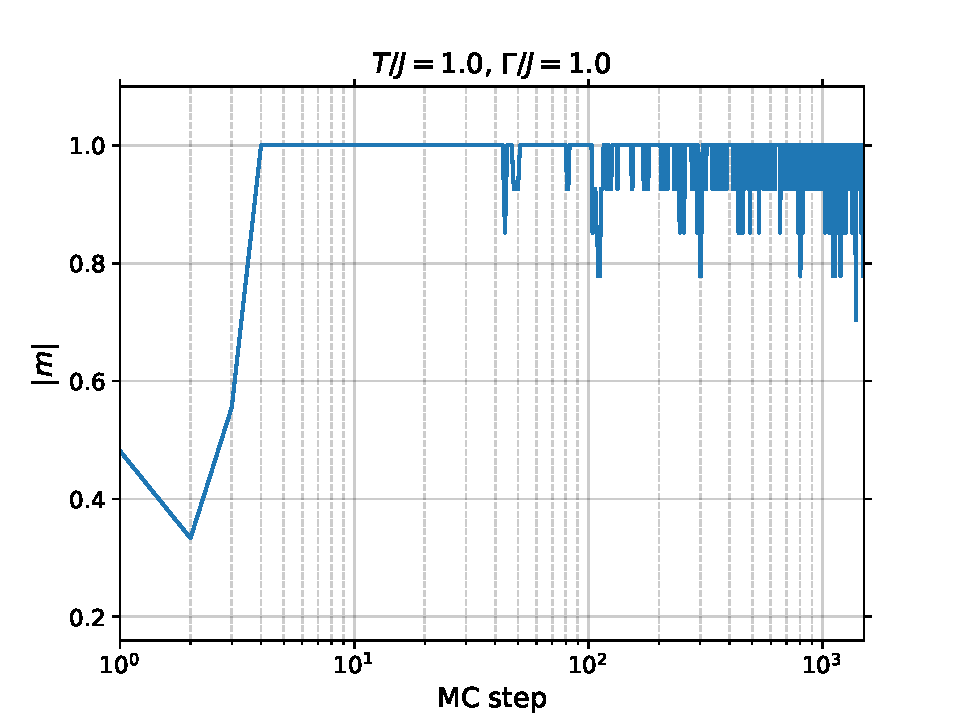
\includegraphics[width=0.5\textwidth]{Plots/MC.pdf}
		\caption{Magnetisation per spin as our Monte-Carlo process goes on at $T/J=1$ and $\Gamma/J=1$ for a $3\times3\times3$ lattice. One MC step represents a whole sweep of the lattice.}
		\label{fig:MC}
	\end{figure}
	
\end{frame}

\section{Results}

\begin{frame}{Trotter dimension size}
	
	\begin{figure}
		\centering
		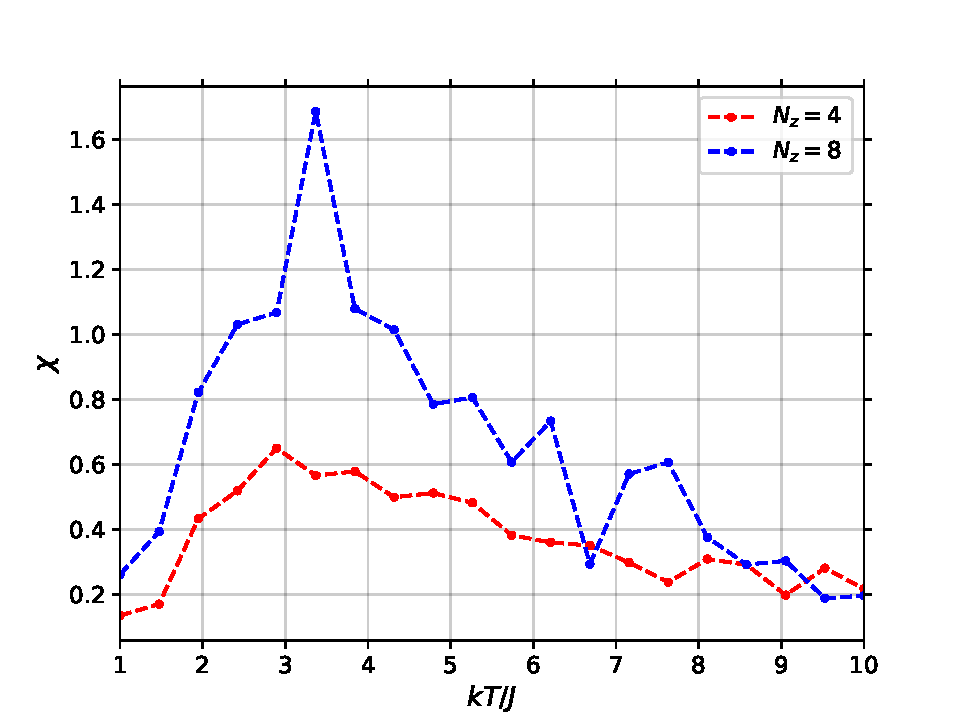
\includegraphics[width=0.5\textwidth]{Plots/T_transition_chi_nz.pdf}
		\caption{Susceptibility as a function of temperature for $\Gamma/J=1$ for a $2\times2\times N_z$ lattice.}
		\label{fig:transition_chi_nz}
	\end{figure}
	
\end{frame}


\begin{frame}{Thermal phase transition}
	
	\begin{figure}
		\centering
		\begin{subfigure}{0.45\textwidth}
			\centering
			\label{fig:T_m}
			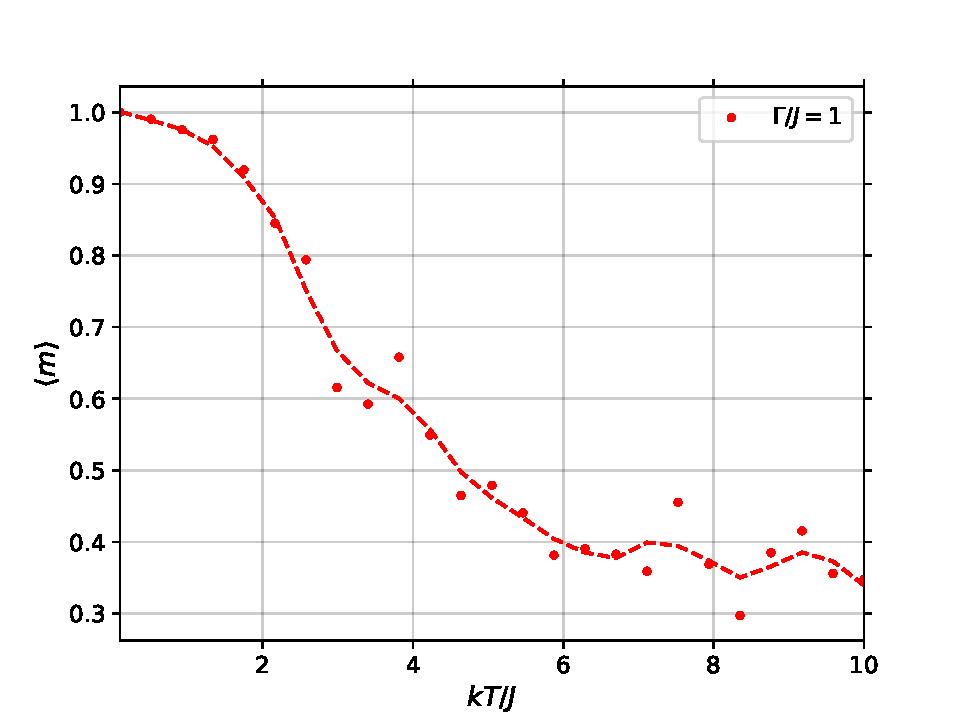
\includegraphics[width=\textwidth]{Plots/T_transition_m.pdf}
		\end{subfigure}
		\begin{subfigure}{0.45\textwidth}
			\centering
			\label{fig:T_chi}
			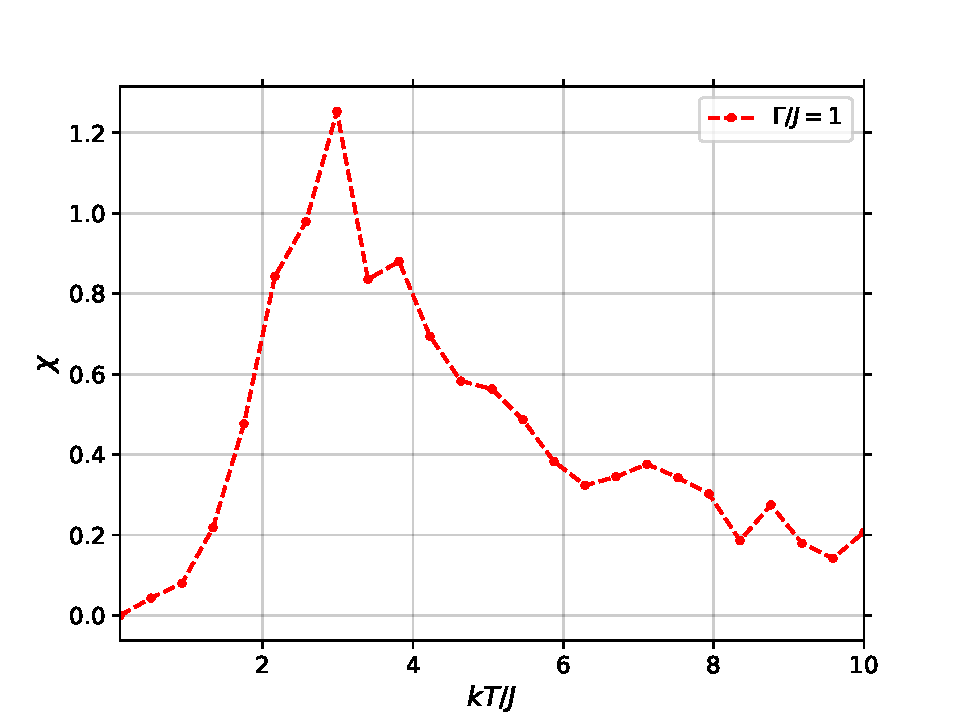
\includegraphics[width=\textwidth]{Plots/T_transition_chi.pdf}
		\end{subfigure}
		\caption{$3\times3\times4$ lattice at $\Gamma/J=1$}
		\label{fig:T_transition}
	\end{figure}
	
\end{frame}


\begin{frame}{Quantum phase transitions}
	
	\begin{figure}[H]
		\centering
		\begin{subfigure}{0.45\textwidth}
			\centering
			\label{fig:gamma_m_T}
			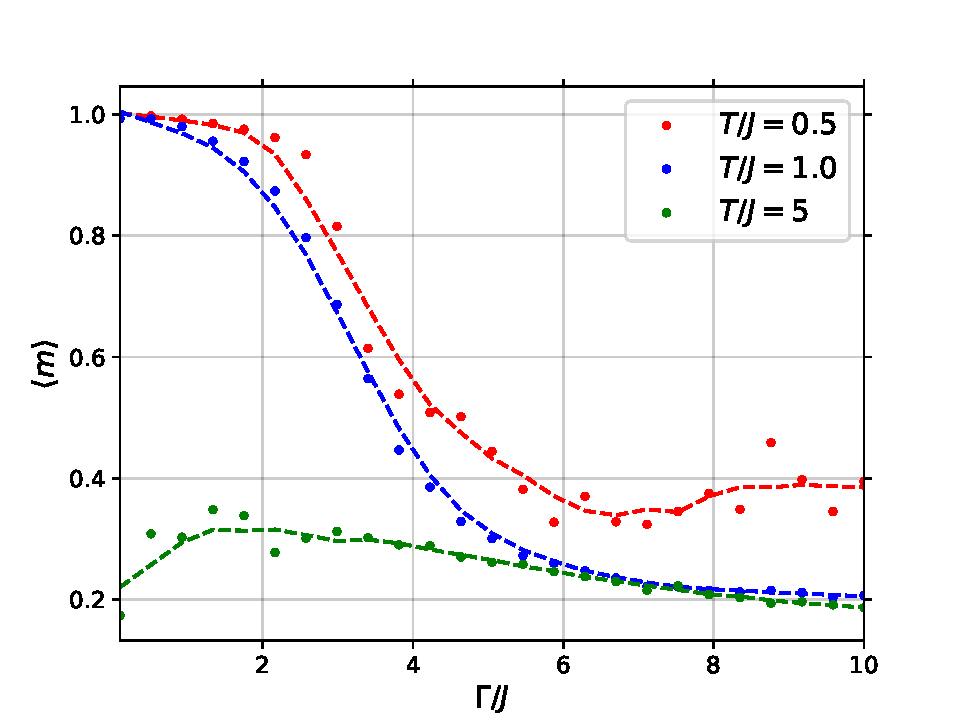
\includegraphics[width=\textwidth]{Plots/gamma_transition_m_T.pdf}
		\end{subfigure}
		\begin{subfigure}{0.45\textwidth}
			\centering
			\label{fig:gamma_chi_T}
			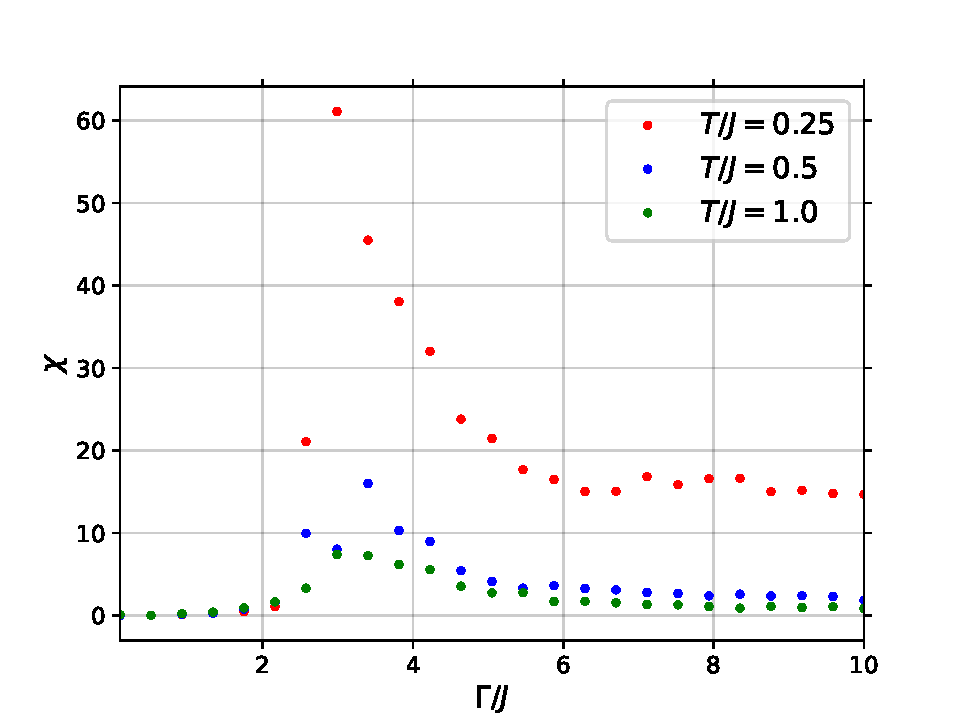
\includegraphics[width=\textwidth]{Plots/gamma_transition_chi_T.pdf}
		\end{subfigure}
		\caption{$4\times4\times10$ lattice}
		\label{fig:gamma_transition_T}
	\end{figure}

\end{frame}


\begin{frame}{Closing remarks}
	
	\begin{itemize}
		\itemsep 1cm
		
		\item A quantum system can be mapped to a classical one with one additional dimension.
		
		\item The size of the additional dimensions has to be large for the mapping to work $\Rightarrow$ limitations due to the slowness of our algorithm.
		
		\item There are numerous other methods for probing $T=0$ phase transitions.
		
		\item There exists a nice link between gauge theories on the lattice and classical statistical mechanics.
	\end{itemize}
	
	
	
\end{frame}


\begin{frame}{References}
	\printbibliography
\end{frame}



\end{document}